\documentclass[10pt,a4paper]{article}
\usepackage[T1]{fontenc}
\usepackage[utf8]{inputenc}
\usepackage{float}
\usepackage{ucs}
\usepackage[top=2cm, bottom=2cm, left=3cm, right=2cm]{geometry}
\usepackage{setspace}
\usepackage{indentfirst}
\usepackage{exsheets}
\SetupExSheets[question]{type=exam}
\usepackage[document]{ragged2e}
\usepackage{fancyhdr}
\usepackage{hyperref}
\usepackage{indentfirst}
\usepackage{setspace}
\usepackage{cmap}
\usepackage{listings}  
\begin{titlepage}
    \author{\Large Danilo Medeiros Eler\\ \Large Gilmar Francisco de Oliveira Santos}
    \title{Universidade Estadual Paulista - UNESP\\Faculdade de Ciências e Tecnologia\\Departamento de Matemática e Computação\linebreak \linebreak \linebreak \linebreak\linebreak \linebreak \linebreak \linebreak
        \Huge Análise sobre Algoritmos de Ordenação \linebreak \Large Projeto e Análise de Algoritmos\linebreak \linebreak \linebreak \linebreak\linebreak\linebreak\linebreak\linebreak\linebreak\linebreak\linebreak\linebreak\linebreak\linebreak\linebreak\linebreak\linebreak\linebreak\linebreak\linebreak\linebreak\linebreak}
    \date{2018\\Outubro}

\end{titlepage}

\renewcommand*\contentsname{Sumário}
\begin{document}
\clearpage\maketitle
\thispagestyle{empty}

\newpage
\thispagestyle{empty}
\tableofcontents

\setlength{\parindent}{4ex}
\newpage
\pagestyle{fancyplain} 
\fancyhf{}
\rhead{\footnotesize Despartamento de Matemática e Computação - DMC}
\lhead{\footnotesize Universidade Estadual Paulista - UNESP}
\rfoot{\thepage}

\section{Introdução}
    \doublespace
    \indent Os Algoritmos de ordenação tem como propósito organizar dados de entrada, geralmente um vetor, rearranjar os elementos e devolver o mesmo em uma determinada ordem, geralmente empregado para valores numéricos ou léxicos, os colocando do menor para o maior ou vice-versa, porém expansível  para diversos tipo de dados.\\
    \indent A ordenação é muito relevante computacionalmente, visto a sua necessidade em muitos dos algoritmos de busca e dentre outras aplicações. A lista de algoritmos de ordenação é bastante extensa, mediante a existência de aplicações aos mais diversos casos, ou mesmo versões melhoradas e variações de um mesmo algoritmo.\\
    \indent A operações básicas presentes nesse tipo de algoritmo geralmente são a comparação de valores, cópia o swap. A \textbf{Complexidade Espacial} é um importante assunto a ser tratado sobre algoritmos de ordenação; alguns necessitam que o vetor de entrada seja copiado e outros ordenam no próprio vetor (in-place) tudo isso influência não só no tempo de execução do mesmo, mas também na quantidade de memória gasta. A \textbf{Estabilidade} é a característica onde dois objetos com as mesmas chaves aparecem na mesma ordem no vetor de entrada, e continuam na mesma ordem no vetor de saída. Neste trabalho a \textbf{Complexidade de Tempo} estará em enfoque.

\newpage
\section{Bubblesort Original}
    \indent Algoritmo de ordenação por flutuação: o que é mais "denso" se deposita no fundo e o que é mais leve flutua. Em seus 3 casos ele executa em $O$(n\textsuperscript{2}) \cite{owen}. É um algoritmo de fácil implementação, que pode ser utilizado para um "n" pequeno, ao passo que a sua complexidade espacial é O(1), ou seja, não utiliza mais que o espaço do próprio vetor para realizar a ordenação, porém para vetores de maior tamanho o algoritmo torna-se muito custoso, visto sua complexidade quadrática. Na análise experimental foi claramente notável a semelhança entre os 3 casos, a única diferença é um gasto menor de tempo para entradas ordenas, visto que não é necessário que os elementos sejam trocados, apenas verificações.
    \begin{figure}[H]
    	\centering
    	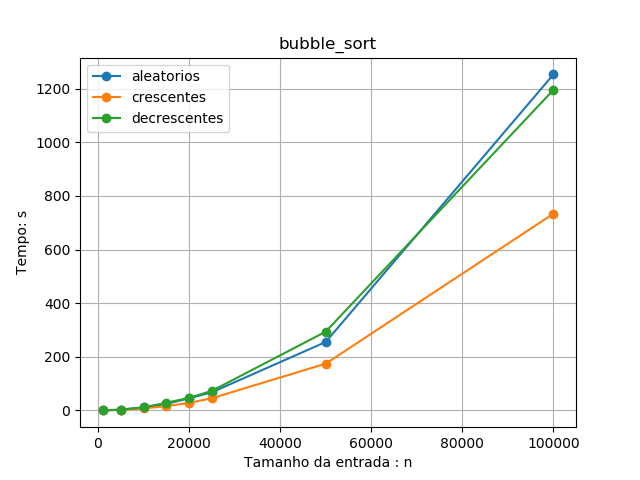
\includegraphics[width=0.58\textwidth]{Resultados/Graficos/bubble_sort.png}
    	\caption{Resultado Bubblesort clássico}
    \end{figure}

\section{Bubblesort Melhorado}
    \indent Adicionado a verificação se o vetor já está ordenado, nesta situação o melhor caso do algoritmo torna-se $\Omega$(n). e os demais casos continuam sendo O(n\textsuperscript{2}).
    \begin{figure}[H]
    	\centering
    	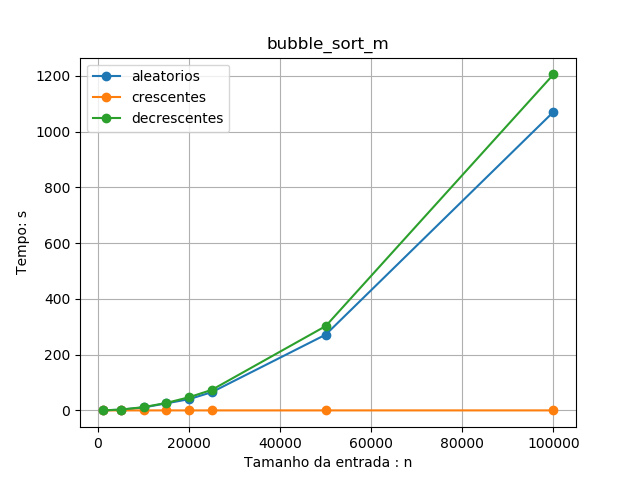
\includegraphics[width=0.58\textwidth]{Resultados/Graficos/bubble_sort_m.png}
    	\caption{Resultado Bubblesort Melhorado}
    \end{figure}

\section{Quicksort}
    \indent Algoritmo que tem base na divisão e conquista, tem o seu melhor caso sendo $\Omega$(n log(n)), seu caso médio é $\Theta$(nlog(n)) e seu pior caso em $O$(n\textsuperscript{2}) \cite{hoare}. É um bom algoritmo para dados aleatórios, o que explica sua grande popularidade, porém seu pior caso ocorre quando é escolhido de forma equivocada o pivô, sendo ele o maior elemento ou o menor elemento, o que acontece é que as partições ficam com tamanhos muito diferentes levando a ineficiência do algoritmo. Sua complexidade espacial é $O$(log(n)), visto que cria partições menores do vetor original.
    \begin{figure}[H]
    	\centering
    	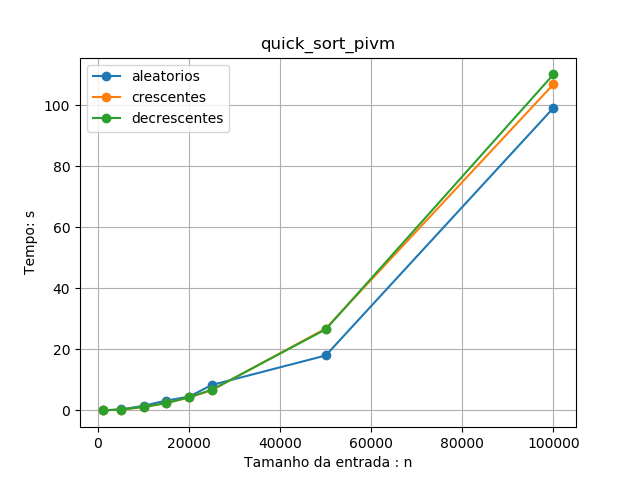
\includegraphics[width=0.63\textwidth]{Resultados/Graficos/quick_sort_pivm.png}
    	\caption{Resultado Quicksort pivô elemento do meio: 3 casos semelhantes}
    \end{figure}
    \begin{figure}[H]
    	\centering
    	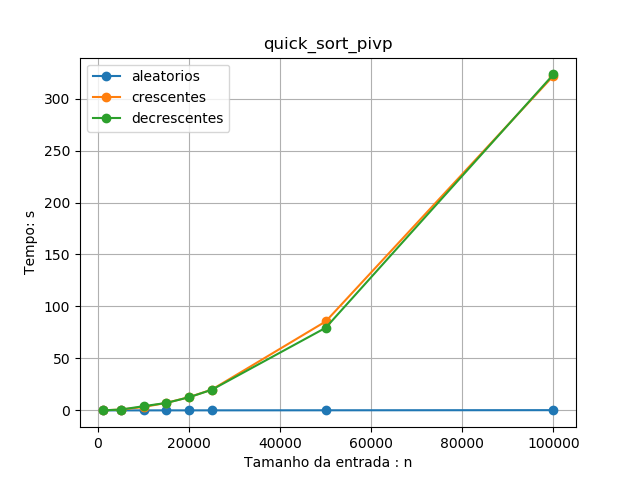
\includegraphics[width=0.63\textwidth]{Resultados/Graficos/quick_sort_pivp.png}
    	\caption{Resultado Quicksort pivô primeiro elemento: acontece o melhor caso, onde as partições tem tamanhos semelhantes.}
    \end{figure}

\section{Mergesort}
    \indent É um algoritmo que utiliza do principio da divisão e conquista para realizar a ordenação. Tem o seu melhor caso $\Omega$(nlog(n)), seu caso médio em $\Theta$(nlog(n)) e seu pior caso em $O$(nlog(n)), o que o faz ser considerado estável \cite{qin}. Porém apresenta uma complexidade espacial de $O$(n), visto as divisão e depois união das partes (conquista) necessárias para a ordenação. Podemos observar que os seu 3 casos são iguais, o que mostra que o mergesort é não sensível a entrada [Ver abaixo], pois realiza sempre particionamentos de mesmo tamanho.  
    \begin{figure}[H]
    	\centering
    	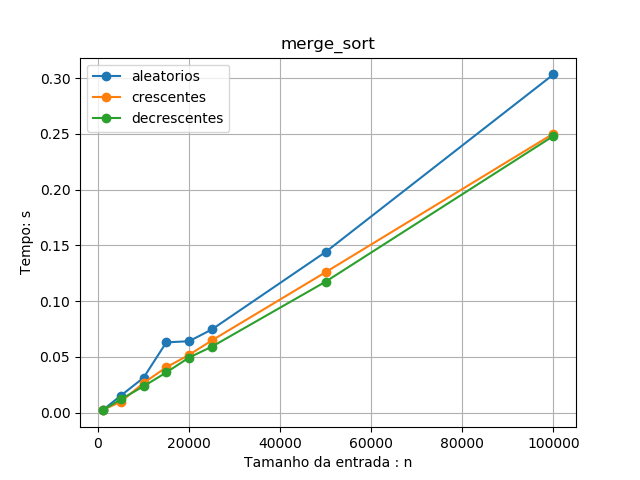
\includegraphics[width=0.5\textwidth]{Resultados/Graficos/merge_sort.png}
    	\caption{Resultado Mergesort: tempos de ordenação muito semelhantes para todos os casos.}
    \end{figure}

\section{Heapsort}
    \indent Utiliza da estrutura de heap para realizar a ordenação. Apresenta melhor caso, caso médio e pior caso proporcionais a $O$(nlog(n)) \cite{schaffer}, o que demonstra que o mesmo é não sensível a entrada, pois executa de maneira semelhante tanto para entradas ordenadas, quanto aleatórias [Ver abaixo]. Como realiza a ordenação utilizando o próprio vetor original, a sua complexidade espacial é de $O$(1).
    \begin{figure}[H]
    	\centering
    	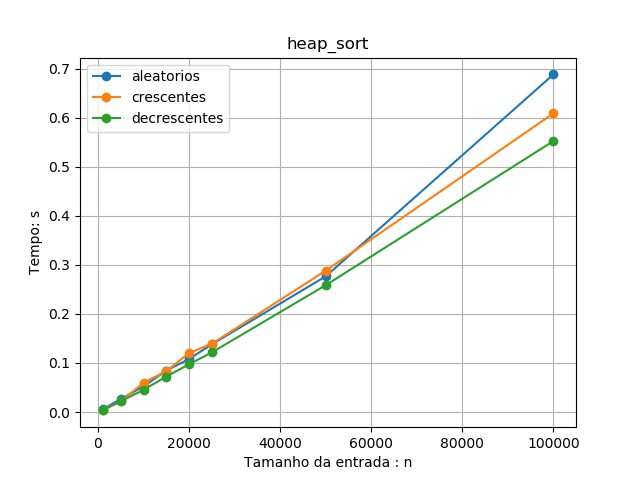
\includegraphics[width=0.5\textwidth]{Resultados/Graficos/heap_sort.png}
    	\caption{Resultado Heapsort}
    \end{figure}

\section{Insertionsort}
    \indent Utiliza da ideia da inserção em uma fila ordenada. Apresenta melhor caso sendo $\Omega$(n); o qual ocorre para vetores ordenados ou parcialmente ordenados, seu caso médio e pior caso são iguais a $O$(n\textsuperscript{2}) \cite{tarundeep}, pois não trabalha muito bem com vetores aleatórios. Como a "inserção" é realizada no próprio vetor, a sua complexidade espacial é de $O$(1).
    \begin{figure}[H]
    	\centering
    	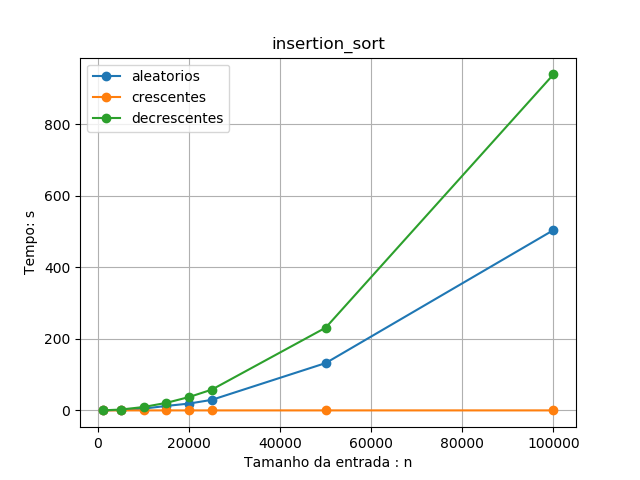
\includegraphics[width=0.63\textwidth]{Resultados/Graficos/insertion_sort.png}
    	\caption{Resultado Insertionsort: melhor caso ocorre para entradas crescentes, enquanto o pior caso ocorre para entradas decrescentes.}
    \end{figure}

\section{ShellSort}
    \indent É um melhoramento do Insetionsort que tem apresenta um gap maior que 1 elemento, seu melhor caso corresponde a $\Omega$(nlog(n)) e ocorre para entradas quase ordenadas, enquanto seu caso médio e pior caso são iguais $\Theta$(n(log\textsuperscript{2}(n)) ou  conforme Sedgewick  $O$(n\textsuperscript{4/3}) no pior caso \cite{sedgewick}. Sua complexidade espacial fica em $O$(1). Nesse trabalho foi utilizada a sequência de Ciura, que se mostrou experimentalmente melhor que as outras sequências de gap como a de Sedgewick. \cite{ciura}.
    \begin{figure}[H]
    	\centering
    	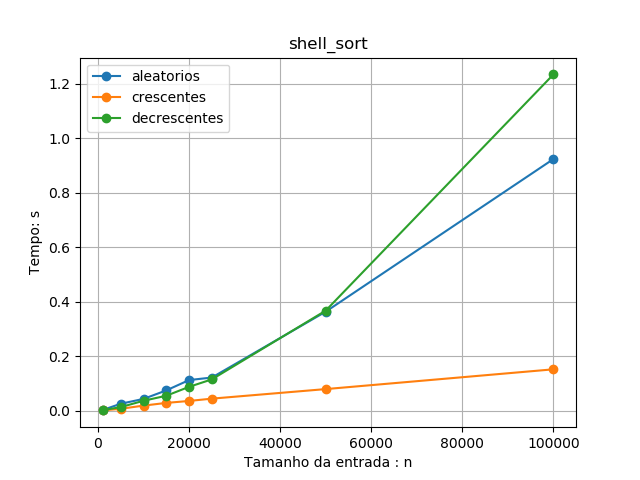
\includegraphics[width=0.5\textwidth]{Resultados/Graficos/shell_sort.png}
    	\caption{Resultado Shellsort para sequência de gaps [701, 301, 132, 57, 23, 10, 4, 1]}
    \end{figure}

\section{Selectionsort}
    \indent O algoritmo utiliza o princípio de sempre encontrar o menor elemento e o colocar em sua posição adequada no vetor. Ele é semelhante ao Bubblesort sem melhoria. Sendo seus 3 casos proporcionais a $O$(n\textsuperscript{2}) \cite{sunita}. Experimentalmente ele apresenta vantagem sobre o Bubblesort. E é um algorítimo muito estável para qualquer tipo de entrada, como é possível observar abaixo:
    \begin{figure}[H]
    	\centering
    	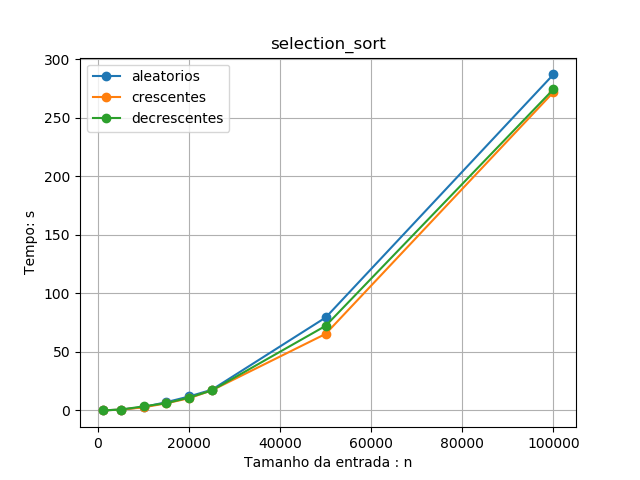
\includegraphics[width=0.5\textwidth]{Resultados/Graficos/selection_sort.png}
    	\caption{Resultado Selectionsort}
    \end{figure}

\newpage
\section{Método}
    \indent Utilizando o linguagem python foram gerados 3 tipos de arquivos para cada quantidade de dados, ordenados: crescente, decrescente e aleatórios, os arquivos referentes ao teste experimental podem ser baixados em htt://git.com. Para o teste experimental foi feita a leitura dos inteiros salvos anteriormente nos arquivos e carregados em vetores na memória (para que a ordenação pudesse ser realizada mais rapidamente, esse processo foi realizado antes da medida do tempo para que não ocorressem interferências na análise). E cada vetor (tamanho, tipo) for submetido a ordenação pelos algoritmos decritos anteriormente e o tempo de execução medido com recisão de 15 casa decimais.\\
    \indent Na seção de Resultados Experimentais constam as tabelas com os tempos de ordenação, que para a melhor visualização apresentam precisão de 4 casas. Utilizando da Biblioteca matplot e os resultados obtidos, foram gerados os gráficos que constam na seção de <Resultados Experimentais>.

    \subsection{Hardware e Software utilizados nos testes Experimentais}
        \begin{flushleft}
            \begin{itemize}
            \item Processador: Intel Core i7-7700HQ CPU @ 2.80GHz x 8 
            \item RAM: 16GB Kingston
            \item SO: Ubuntu 16.04.5 LTS 64-bit Gnome3
            \item Editor de Texto: VS Code v1.28.1
            \item Linguagem: Python 3.5.2 64-bit
            \item Bibliotecas: Numpy v1.15.1, Scypy v1.1.0, matplotlib v3.0.0.
        \end{itemize}
        \end{flushleft}

\newpage
\section{Resultados Experimentais}
    \indent Para o catálogo e geração de gráficos foi utiliza a biblioteca matplot do python (Ver descrição de Hardware e Software). Os arquivos texto com os resultados estão salvos na pasta de "Resultados", presente no repositório.
    \subsection{Entradas Aleatórias}
        \indent Para entrada de dados aleatória é facilmente notável que algoritmos como o Quicksort, ShellSort ou outros algoritmos baseados em divisão e conquista e particionamento são os mais indicados:
        \begin{center}
            \begin{table}[H]
                \begin{tabular}{l*{9}{c}r}

                    \textbf{Algoritmo}      & \multicolumn{8}{ c }{\textbf{Número de elementos do vetor}} \\ \cline{2-9}
                    & \textbf{1000}& \textbf{5000} & \textbf{10000} & \textbf{15000} & \textbf{20000} & \textbf{25000} & \textbf{50000} & \textbf{100000} \\ \cline{1-9}
                    \textbf{bubbleSort}     & 0.1205    & 2.6833    & 11.3439   & 24.6648   & 45.0675   & 67.7314   & 255.3029  & 1253.3219\\
                    \textbf{bubbleSortM}    & 0.1027    & 2.5444    & 10.5627   & 25.2195   & 40.2927   & 65.4530   & 271.7309  & 1070.5516\\
                    \textbf{heapSort}       & 0.0057    & 0.0263    & 0.0523    & 0.0843    & 0.1081    & 0.1379    & 0.2765    & 0.6880\\
                    \textbf{insertionSort}  & 0.0594    & 1.3235    & 4.9474    & 12.4794   & 19.0760   & 29.5371   & 132.2940  & 503.8637\\
                    \textbf{MergeSort}      & 0.0021    & 0.0152    & 0.0313    & 0.0630    & 0.0640    & 0.0746    & 0.1441    & 0.3034\\
                    \textbf{QuickSortPivM}  & 0.0080    & 0.3138    & 1.5135    & 3.2253    & 4.5025    & 8.3376    & 17.989    & 99.0538\\
                    \textbf{QuickSortPivP}  & 0.0017    & 0.0168    & 0.0231    & 0.0369    & 0.0408    & 0.0627    & 0.1124    & 0.2402\\
                    \textbf{SelectionSort}  & 0.0339    & 0.7289    & 2.8884    & 7.0576    & 11.930    & 17.681    & 79.410    & 287.0386\\
                    \textbf{ShellSort}      & 0.0026    & 0.0257    & 0.0435    & 0.0747    & 0.1126    & 0.1219    & 0.3636    & 0.9235\\
                    \hline
                \end{tabular}
                \caption{Resultados em segundos dos algoritmos de ordenação para dados aleatórios}
            \end{table}
            \begin{figure}[H]
                \centering
                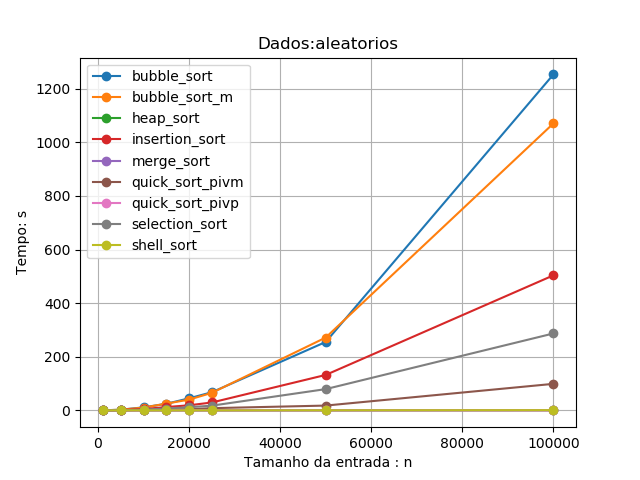
\includegraphics[width=0.63\textwidth]{Resultados/Graficos/aleatorios.png}
                \caption{Resultado para entrada de dados aleatória}
            \end{figure}
        \end{center}
    
    \subsection{Entradas Ordenadas Crescentemente}
    \indent Entradas crescentes geralmente geram melhores casos para algoritmos muito sensíveis a entrada, como o Bubblesort Melhorado e insertionSort.
    \begin{center}
        \begin{table}[H]
            \begin{tabular}{l*{9}{c}r}
                \textbf{Algoritmo}      & \multicolumn{8}{ c }{\textbf{Número de elementos do vetor}} \\ \cline{2-9}
                & \textbf{1000}& \textbf{5000} & \textbf{10000} & \textbf{15000} & \textbf{20000} & \textbf{25000} & \textbf{50000} & \textbf{100000} \\ \cline{1-9}
                \textbf{bubbleSort}     & 0.0920    & 1.8210    & 7.3573    & 16.417    & 27.8725   & 45.5481   & 174.3917  & 733.9344\\
                \textbf{bubbleSortM}    & 0.0001    & 0.0004    & 0.0007    & 0.001     & 0.0015    & 0.0020    & 0.0037    & 0.0134\\
                \textbf{heapSort}       & 0.0050    & 0.0215    & 0.0598    & 0.083     & 0.1202    & 0.1391    & 0.2880    & 0.6086\\
                \textbf{insertionSort}  & 0.0001    & 0.0005    & 0.0009    & 0.001     & 0.0021    & 0.0026    & 0.0050    & 0.0155\\
                \textbf{MergeSort}      & 0.0024    & 0.0096    & 0.0266    & 0.040     & 0.0518    & 0.0647    & 0.1260    & 0.2502\\
                \textbf{QuickSortPivM}  & 0.0177    & 0.2748    & 1.0689    & 2.403     & 4.2333    & 6.6343    & 26.8120   & 106.8023\\
                \textbf{QuickSortPivP}  & 0.0360    & 0.8027    & 3.2692    & 7.230     & 12.7422   & 20.0302   & 85.5832   & 321.9686\\
                \textbf{SelectionSort}  & 0.0277    & 0.7007    & 2.6305    & 6.094     & 10.4270   & 17.1721   & 65.4112   & 271.9045\\
                \textbf{ShellSort}      & 0.0013    & 0.0072    & 0.0189    & 0.028     & 0.0360    & 0.0444    & 0.0795    & 0.1520\\
                \hline
            \end{tabular}
            \caption{Resultados em segundos dos algoritmos de ordenação para dados crescentes}
        \end{table}
        \begin{figure}[H]
            \centering
            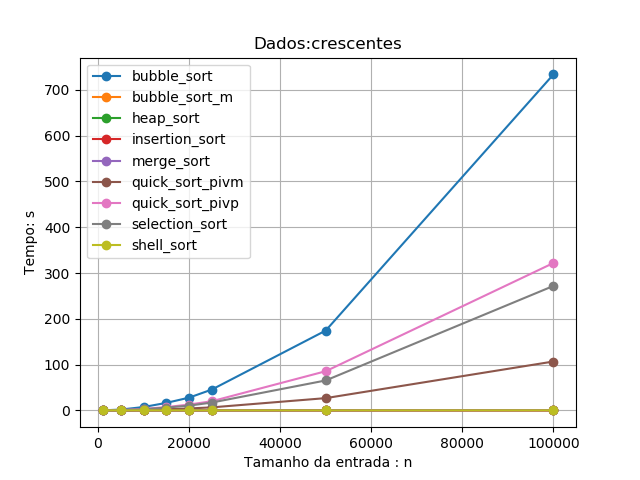
\includegraphics[width=0.63\textwidth]{Resultados/Graficos/crescentes.png}
            \caption{Resultado para entrada de dados crescente}
        \end{figure}
    \end{center}
    
    \subsection{Entradas Ordenadas Decrescentemente}
    \indent Entradas ordenadas de maneira descrescente fazem com que vários dos algoritmos atinjam seus piores casos, o que é evidenciado pela elevação do teto para 1200s.
    \begin{center}
        \begin{table}[H]
            \begin{tabular}{l*{9}{c}r}
                \textbf{Algoritmo}      & \multicolumn{8}{ c }{\textbf{Número de elementos do vetor}} \\ \cline{2-9}
                & \textbf{1000}& \textbf{5000} & \textbf{10000} & \textbf{15000} & \textbf{20000} & \textbf{25000} & \textbf{50000} & \textbf{100000} \\ \cline{1-9}
                \textbf{bubbleSort}     & 0.1575    & 2.9523    & 11.5620   & 28.5389    & 46.9204   & 73.0083   & 293.8050  & 1195.6926\\
                \textbf{bubbleSortM}    & 0.1409    & 2.9037    & 11.6687   & 26.7478    & 47.2076   & 73.7579   & 302.4040  & 1205.0179\\
                \textbf{heapSort}       & 0.0033    & 0.0220    & 0.0450    & 0.0723     & 0.0973    & 0.1215    & 0.2584    & 0.5521\\
                \textbf{insertionSort}  & 0.1078    & 2.3851    & 9.4417    & 21.0452    & 37.3525   & 58.1049   & 231.2657  & 939.0387\\
                \textbf{MergeSort}      & 0.0020    & 0.0119    & 0.0236    & 0.0360     & 0.0494    & 0.0591    & 0.1175    & 0.2482\\
                \textbf{QuickSortPivM}  & 0.0151    & 0.2881    & 1.1517    & 2.4017     & 4.3101    & 6.7552    & 26.5462   & 110.0228\\
                \textbf{QuickSortPivP}  & 0.0402    & 0.8008    & 4.0329    & 7.1814     & 12.6456   & 19.8759   & 79.5031   & 323.2435\\
                \textbf{SelectionSort}  & 0.0332    & 0.7067    & 3.4609    & 6.2206     & 10.9902   & 17.0810   & 72.2877   & 274.3372\\
                \textbf{ShellSort}      & 0.0019    & 0.0134    & 0.0366    & 0.0551     & 0.0877    & 0.1152    & 0.3674    & 1.2341\\
                \hline
            \end{tabular}
            \caption{Resultados em segundos dos algoritmos de ordenação para dados descrescentes}
        \end{table}
        \begin{figure}[H]
            \centering
            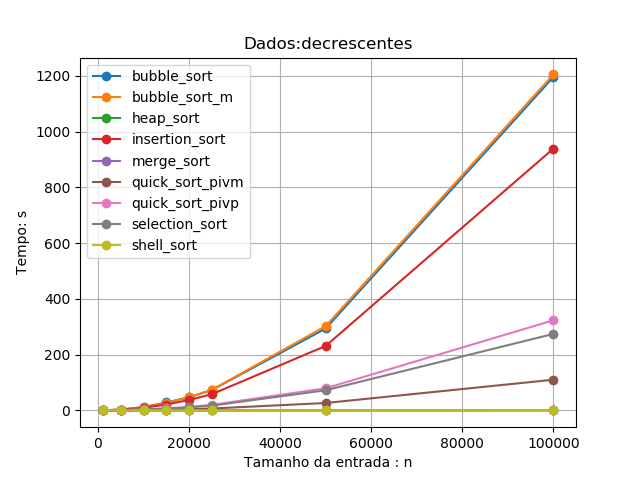
\includegraphics[width=0.63\textwidth]{Resultados/Graficos/decrescentes.png}
            \caption{Resultado para entrada de dados descrescente}
        \end{figure}
    \end{center}

\newpage
\section{Conclusão}
    \indent O melhor algoritmo para casos genéricos; vetores aleatórios e de maiores tamanhos, ou mesmo entradas ordenadas se mostrou experimentalmente ser o ShellSort, neste caso utilizando a sequência de Ciura, porém se faz necessário analisar com extremo cuidado cada caso em que se trabalha, para verificar se existe algum algoritmo de ordenação que faz mais sentido a situação problema, sempre tendo em mente o uso balanceado dos recursos, para maximizar a eficência dos sistemas computacionais. \\
    \indent Em contra ponto o Bubblesort original tem um custo maior até mesmo que os algoritmos com mesma complexidade como o Insertionsort, seu uso deve ser evitado sempre que possível.

\newpage
\pagestyle{empty} 
\renewcommand\refname{Referências}
\begin{thebibliography}{9}

	\bibitem{ciura}
	Marcin Ciura,
	\textit{Best Increments for the Average Case of Shellsort},
    2001.

    \bibitem{sedgewick}
	Sedgewick, R.,
	\textit{Analysis of Shellsort and Related Algorithms},
    1996.
    
    \bibitem{owen}
	Owen Astrachan,
	\textit{Bubble Sort: An Archaeological Algorithmic Analysis},
	2003.
    
    \bibitem{bell}
	D. A. Bell,
	\textit{The Principles of Sorting},
	1958.
    
    \bibitem{knowles}
	Joshua Knowles,
	\textit{Sorting Algorithms: Correctness, Complexity and Other Properties},
	2013.
    
    \bibitem{hoare}
	C. A. R. Hoare,
	\textit{Quicksort},
	1962.
    
    \bibitem{qin}
	Song Qin,
	\textit{Merge Sort Algorithm }
    
    \bibitem{schaffer}
	Schaffer R, Sedgewick R.,
	\textit{The Analysis of Heapsort},
	2002.
    
    \bibitem{tarundeep}
	Tarundeep S. S., Surmeet K., Snehdeep K.,
	\textit{Enhanced Insertion Sort Algorithm},
	2013.
    
    \bibitem{sunita}
	Sunita C., Teshu C., Rubina P,
	\textit{Upgraded Selection Sort},
	2011.
\end{thebibliography}
	
\end{document}
	